\section{Confined Compression Test.}
\label{excomp}
A second common test conducted on soft material is confined compression. As illustrated in Figure \ref{confcomp}, a porous plate is used so that the fluid is free to flow and the chemical equilibrium with the external bath is restored after the transient relaxation phase. After gradual compression of the tissue, the system is allowed to relax while the strain $\epsilon$ is maintained constant \cite{Netti}. We here interested in the equilibrium, i.e. relaxed, behaviour of the sample, which is described by a stress-strain curve (see Figure \ref{fit} as an example). 

\begin{figure}[h]
	\centering
	\def\svgwidth{0.89\linewidth}
	\input{latex/images/compression.pdf_tex}
	\vspace{2mm}
	\caption{Schematic representation of a compression test with a porous piston. A deformation is imposed in the $Z$ direction and the force necessary to maintain the deformation is recorded. }
	\label{confcomp}
\end{figure}

As we consider a swollen slice of tissue compressed in the $Z$ direction, the deformation $\F$ from the dry to the current state has the form:

\begin{equation}
\F=J_0^{1/3}\begin{bmatrix}
1 &0&0\\
0&1&0\\
0&0& \lambda_1
\end{bmatrix},
\label{F} 
\end{equation}
where $\lambda_1 = 1 - \epsilon$ and $J_0$ defines the initial swollen state. 

As the problem is one-dimensional, we can reduce the number of unknowns. We define $u=\mathbf{u}\,\cdot\,\mathbf{e}_Z$, $T_{zz}= \mathbf{e}_Z \mathbb{T}\mathbf{e}_Z$ and $J_m=\mathbf{J}_m\,\cdot \,\mathbf{e}_Z$, the component of the displacement, deformation tensor and fluxes in the $Z$ direction. Assuming the slice to have an initial height $H_0$, proper boundary conditions need to be assigned at the two edges $Z=0$ and $Z=H_0$:
\begin{eqnarray}
\left[\mu_s\right]^+_-=\left[\mu_+\right]^+_-=\left[\mu_-\right]^+_-=0, \quad \left[T_{zz}\right]^+_-=0, &\qquad& Z=H_0\,,\\
J_m = u = 0, &\qquad& Z=0\, ,\\
\frac{\d \Phi}{\d Z}=0 &\qquad& Z=0,H_0\,.
\end{eqnarray}

At equilibrium, the conditions~1 and 2 listed in Section \ref{free} still hold. On the other hand, due to the external force $\mathbf{F}= -F_z \mathbf{e}_z$ which is exerted on the plate of area $A$, condition 3 now reads:

\begin{equation}
T_{zz}=\sigma = -\frac{F_z}{A}.
\end{equation} 

\subsection{Model Comparison.}
\label{data}
Starting from model A, given the symmetries of the problem, $\B_e$ is a diagonal matrix of the form:
\begin{equation}
\B_e=\begin{bmatrix}
b &0&0\\
0&b&0\\
0&0& b_1
\end{bmatrix}. 
\end{equation}
If we now study the fixed point of Equation~(\ref{Be}), we obtain that $b=b_1=J_0^{2/3}\lambda_1^{2/3}$ as $\det \B_e= (\det \F)^2$.

Focusing on model B instead, the tensors $\bar{\B}$ and $\bar{\B}_e$ are now of the form:
\begin{equation}
\bar{\B}=\begin{bmatrix}
\lambda_1^{-2/3} &0&0\\
0&\lambda_1^{-2/3}&0\\
0&0& \lambda_1^{4/3}
\end{bmatrix}, \qquad
\bar{\B}_e=\begin{bmatrix}
\bar{b} &0&0\\
0&\bar{b}&0\\
0&0& \bar{b}_1
\end{bmatrix}
\end{equation}
with the $\bar{b}=\bar{b}_1=1$ at equilibrium so that the spring $2$ does not contribute to the stress. Substituting the equilibrium conditions into the state equations for the two models (see Table \ref{summary}) yields to:
\begin{gather}
p = \begin{cases}
\displaystyle
-\sigma + \frac{G^A_1}{J_0\lambda_1} (J^{2/3}_0\lambda_1^2-1)+\frac{G^A_2}{J_0\lambda_1} (J_0^{2/3} \lambda_1^{2/3}-1) &\quad \text{MODEL A} \\[10pt]
-\sigma + \dfrac{G_{vol}}{J_0\lambda_1}(J_0^{2/3}\lambda_1^{2/3}-1)+\dfrac{2G^B_1}{3J_0\lambda_1^{5/3}} (\lambda_1^2-1) &\quad \text{MODEL B}
\end{cases}\\[10pt]
\begin{aligned}
\frac{\sigma v_s}{k_B T}=\frac{J_0\lambda_1+\chi}{J_0^2\lambda^2_1}+\frac{pv_s}{k_B T}+&\ln \frac{J_0\lambda_1-1}{J_0\lambda_1} +2c_0v_s\\
-\ &\sqrt{\left(\frac{z_fC_fv_s}{J_0\lambda_1-1}\right)^2+4v_s^2c^2_0}
\end{aligned}\label{compA}
\end{gather}

Unlike for unconstrained swelling, we note that model $A$ and $B$ are now substantially different, as there is no choice of parameter values for which the two are equivalent for any value of $\lambda_1$. 

Following the work of Xue et al~\cite{ecm2}, we test our models on the data collected by Netti et~al. \cite{Netti} on HSTS 26T sarcoma slices. Despite our model being built to describe decellularized ECM, cells can be included in the model simply as part of the solid phase \cite{ecm2}. As we are interested in the tissue scale, this is a good approximation. However, as suggested also by Xue et~al.\cite{ecm2}, more accurate models also incorporate the cellular activities. However, this goes beyond the purpose of our study.

\begin{figure}[h]
	\hspace{-8mm}
	\begin{subfigure}{0.62\textwidth}
		\hspace{2mm}
		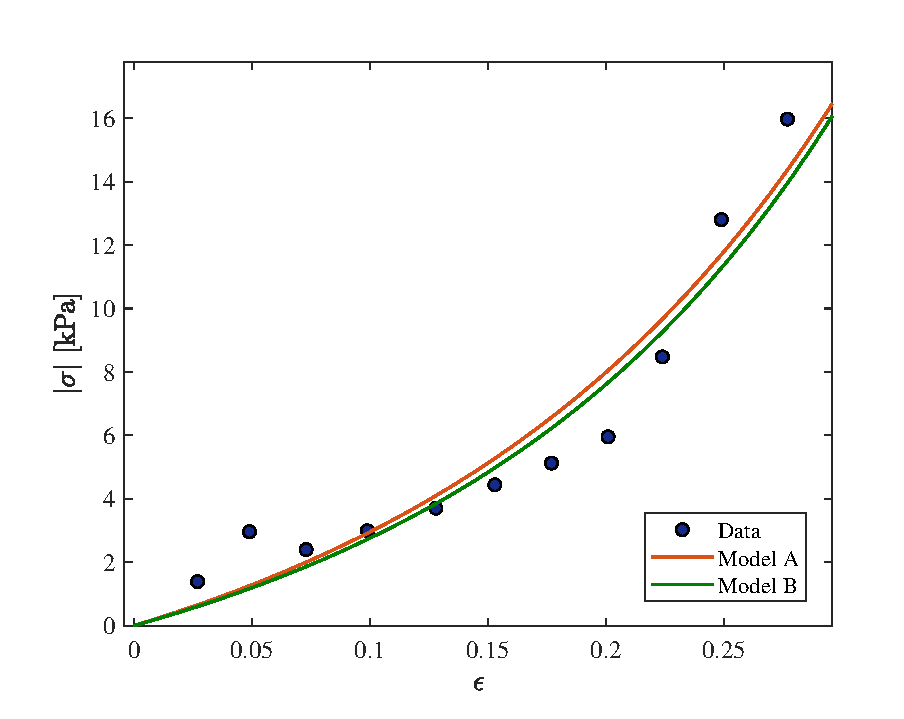
\includegraphics[scale=0.42]{images/compression2.eps}
		\caption{Fitted Model}
		\label{fit}
	\end{subfigure}
	\begin{subtable}{0.375\textwidth}
		\begin{tabular}{c | c ||c| c }		
			\hline\addlinespace[2pt]
			\multicolumn{2}{c||}{Model A} &  \multicolumn{2}{c}{Model B}\\[0.5mm]
			\hline\addlinespace[2pt]
			$\quad \chi\quad$ & $\quad0.498\quad$ &$\quad \chi\quad$&$\quad0.524\quad$\\[0.5mm]
			$G^A_1$ & 18.9 kPa&$G_{vol}$&75 Pa\\[0.5mm]
			$G^A_2$ & 5.3 Pa&$G^{B}_{1}$& 55.1 kPa\\[0.5mm]
			$J_0$ & $20.7$&  $J_0$&$14.8$\\[0.5mm]
			\hline
		\end{tabular}
		\caption{Estimated Parameters}
		\label{param}
	\end{subtable}
	\caption{Comparison of the two models in fitting real experimental data from \cite{Netti}.}		
\end{figure}

Together with the stress-strain curve from the compression test, Netti et~al. measure also the tissue composition, so that $C_f$ is known (see Table \ref{Tab1}). The other parameters listed in Table \ref{Tab1} have been taken from the literature. Consequently the set of unknown parameters is $\left\{\chi, G^A_1, G^A_2\right\}$ and $\left\{\chi, G_{vol}, G^B_1\right\}$ for models A and B respectively. These are estimated fitting Equation~(\ref{compA}) to the data, using the \texttt{fmincon} function in MATLAB, which implements the non-linear least squares method\footnote{the result as been optimized starting from different initial condition, so to explore a larger part of the parameter space}.

As shown in Figure \ref{fit}, both models are able to capture the qualitative behaviour of the data. However they largely disagree in their quantitative predictions, see Table \ref{param}. Let us for example compute the initial pressures in the tissue slice, i.e. $p$ at $\lambda_1=1$:  
\begin{gather}
p_A = \frac{G^A_1+G^A_2}{J_0}(J_0^{2/3}-1) = \frac{24.2 \text{ kPa}}{20.7}(20.7^{2/3}-1) = 7.64 \text{ kPa},\\
p_B = \frac{G_{vol}}{J_0}(J_0^{2/3}-1) = \frac{0.075 \text{ kPa}}{14.8}(14.8^{2/3}-1) = 25.5 \text{ Pa},
\end{gather}
then the two differ of several order of magnitude. Consequently, the models give a completely different estimation of the pressure cells in the tissue are exposed to. As hydrostatic pressure affect cells behaviour \cite{viscocell}, based on which model is considered, we could end up with completely different conclusion on the mechano-sensitivity of cells.
\begin{figure}[h!]
	\begin{subfigure}{0.49\textwidth}
		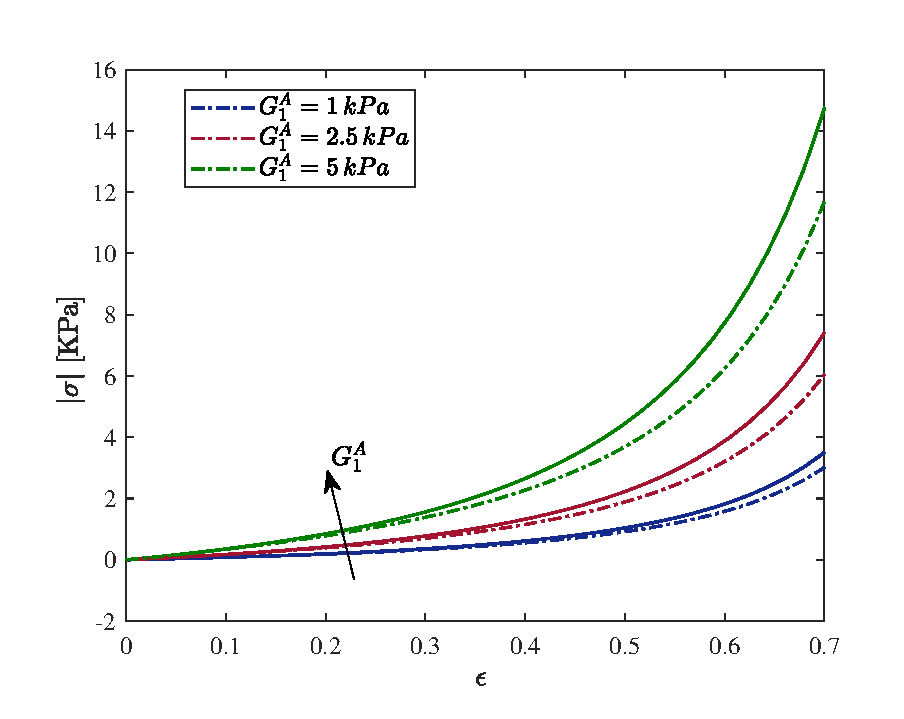
\includegraphics[scale=0.4]{images/comp1}
		\caption{}
	\end{subfigure}
	\begin{subfigure}{0.49\textwidth}
		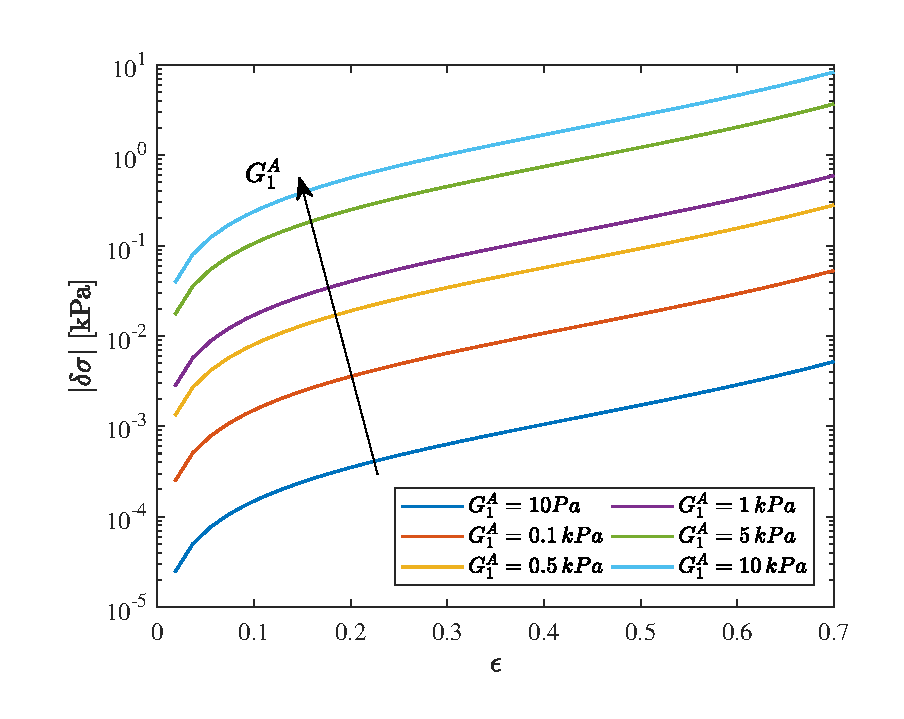
\includegraphics[scale=0.4]{images/comp2}
		\caption{}
	\end{subfigure}
	
	\begin{subfigure}{0.49\textwidth}
		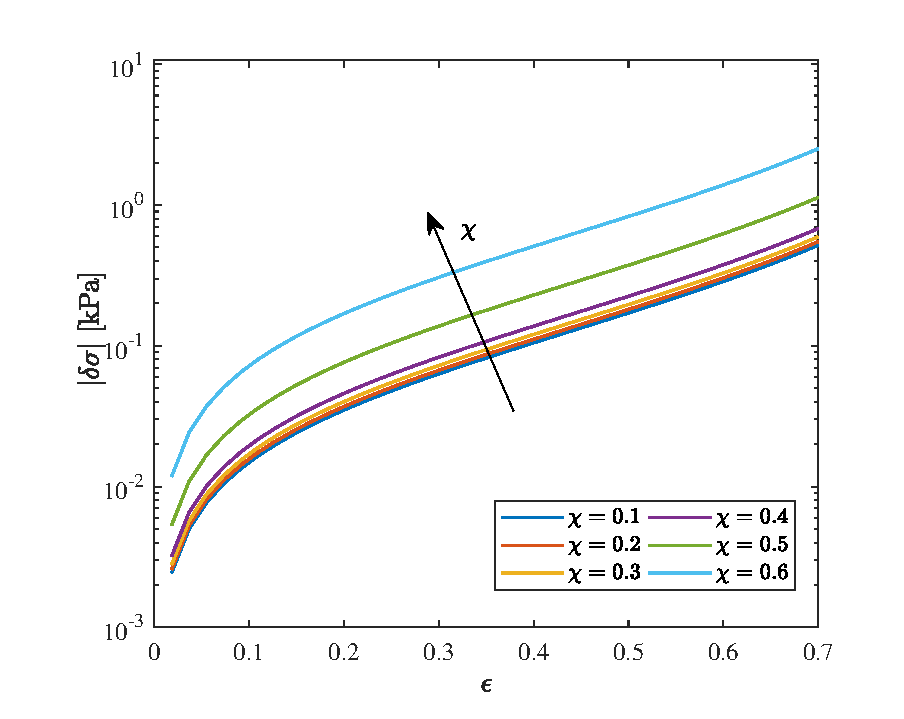
\includegraphics[scale=0.4]{images/comp3}
		\caption{}
	\end{subfigure}
	\begin{subfigure}{0.49\textwidth}
		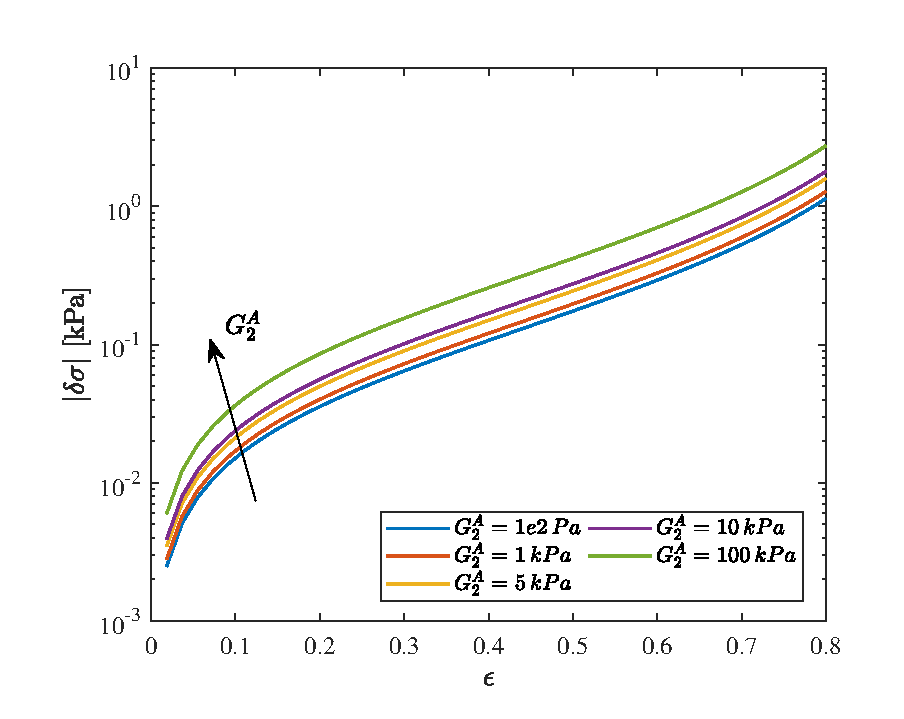
\includegraphics[scale=0.4]{images/comp4}
		\caption{}
	\end{subfigure}
	\caption{Sensitivity Analysis. As expected the mismatch between the two models grows with the strain: (a) Comparison of stress-strain curve predicted by model A (dotted line) and model B (full line) for different values of the parameter $G^A_1$; (b) as $G_1^A$ increases so does the discrepancy $\delta\sigma$; (c) $\delta\sigma$ is also particularly sensitive to changes in the mixing parameter $\chi$, in particular we see that there is a relevant jump when the ECM is in the \textit{collapsed} phase; (d) on the other hand, only large changes in $G^A_2$ have a relevant impact on $\delta\sigma$.}
	\label{comp3}
\end{figure}

Looking at the Table  \ref{param}, we note that $G_{vol}\neq G^A_{1}+G^A_2$, so that, the two estimated models would disagree also in the case of free-swelling. Based on the result from Section \ref{free}, we propose that a two-step protocols which combines free-swelling and compression test can be more informative to identify the material properties. To reproduce this setting \textit{in silico}, we compare again models $A$ and $B$ simulating a compression experiment. This time however we assume that the parameters $\chi$ and $G_{vol}=G^A_{eq}$ are fixed, as if they have been previously estimated by unconstrained swelling experiment. If we now take the difference between the compression stress predicted by Equation~(\ref{compA}) for the two models, i.e. $\delta \sigma= \sigma_{B}-\sigma_{A}$, we obtain:
\begin{equation}
\delta \sigma = \frac{2 G_1^{B}}{3} \frac{\lambda_1^2-1}{J_0\lambda_1^{5/3}} - \frac{G_1^A}{J_0^{1/3}}(\lambda_1-\lambda_1^{-1/3}).\label{err}
\end{equation}
For the purpose of our analysis, we impose the two models to agree at the second order in the regime of small deformation. This translates in the conditions $\lambda_1\rightarrow 1$:
\begin{equation}
\left.\delta \sigma\right|_{\lambda_1=1}=0 \qquad \left.\frac{\d \delta \sigma}{\d \lambda_1}\right|_{\lambda_1=1}=0 \quad\Rightarrow \quad G_1^{B} = J_0^{2/3}G_1^A.\label{temp14}
\end{equation}
Under such conditions we can rewrite Equation~(\ref{err}) as:
\begin{equation}
\delta \sigma(\lambda_1;G^A_1,J_0) = \frac{G_1^A}{J^{1/3}_0\lambda_1^{5/3}} \left(\frac{2}{3}\lambda^2_1-\frac{2}{3}-\lambda_1^{5/3}+\lambda_1^{4/3}\right), 
\end{equation}
where $J_0$ is defined by Equation~(\ref{eqF}). As shown in Figure \ref{comp3}, $\delta \sigma$ is an increasing function of $\epsilon$ as the two model appear to diverge exponentially as $\epsilon \rightarrow 0 $. Consequently, in the large-deformation regime we should be able to distinguish between the two models. Let us consider the case in which $\chi$ and $G_{vol}$ are estimated by free-swelling experiment as in Figure~(\ref{param}). Using Equation~(\ref{temp14}) and the condition $G_{vol}=G^A_{eq}$, we would have that $G^A_2<0$, which is not physically admissible. This is to highlight how, having information about free and constraint swelling can be informative in identifying the proper model. 

We could not find data from the literature for both swelling and compression tests on tissues, so that we can not yet conclude whether both, one or none of the models effectively describe soft tissue. This will require further experimental testing. With this aim, we have also performed a sensitivity analysis on the model parameters. As illustrated in Figure~(\ref{comp3}), $\chi$ and $G_1^A$ are the parameters that have the more impact on $\delta\sigma$. While $G_1^A$ depends only on the properties of the material, $\chi$ can be tuned by changing the temperature $T$ so to optimise the experimental condition. 


%We here consider another standardd
